\chapter{Introducción General}

\label{Chapter1}
\label{IntroGeneral}

%-------------------------------------------------------------------------------

\newcommand{\keyword}[1]{\textbf{#1}}
\newcommand{\tabhead}[1]{\textbf{#1}}
\newcommand{\code}[1]{\texttt{#1}}
\newcommand{\file}[1]{\texttt{\bfseries#1}}
\newcommand{\option}[1]{\texttt{\itshape#1}}
\newcommand{\grados}{$^{\circ}$}

%-------------------------------------------------------------------------------

El capítulo presenta las necesidades a satisfacer y una introducción técnica, con el objetivo de proveer de conceptos básicos para comprender el resto de la memoria.

\section{Motivación}
\label{ch1Motivacion}

% Hacia adonde se dirige la tecnología
% Internet de las cosas 
% Cómo la próxima evolución de Internet lo cambia todo
% Dave Evans
% Abril de 2011
% Cisco Internet Business Solutions Group (IBSG)
% https://www.cisco.com/c/dam/global/es_mx/solutions/executive/assets/pdf/internet-of-things-iot-ibsg.pdf
La tendencia tecnológica actual es interconectar los dispositivos a través de la Internet, a tal punto que la cantidad de objetos en el año 2009 superó al número de personas conectadas, y llegado el 2020 la diferencia es de seis veces en favor de las cosas.
Los procesos industriales se ven beneficiados con nuevos métodos de control de inventarios y análisis de mediciones, además es posible gestionar los ambientes productivos para lograr una mayor calidad y comodidad.
Los datos quedan disponibles para ser procesados por modelos de inteligencia artificial, y la información resultante puede ser vista desde cualquier ubicación y en múltiples plataformas. 

% Realidad de la industria local
% Plan estratégico industrial 2020
Las empresas locales están retrasadas en su progreso tecnológico, muchas no incorporaron sistemas electrónicos en sus procesos o productos, es necesario crear un sistema que logre adaptar la tecnología en uso con el fin de incorporarlas a las nuevas prácticas de negocios.
El avance tecnológico modifica el marco normativo de las naciones, para cumplir con los nuevos requerimientos jurídicos, se necesita tener un mínimo de capital.
El retraso tecnológico ya no solo genera una pérdida de competitividad, sino que también impide que las empresas coloquen sus mercancías en otros países, por incumplimiento en normas de calidad o de protección del medio ambiente.
		
% Necesidades de Gador		
La situación de la industria argentina fue la primera razón que impulsó este trabajo, el siguiente paso fue buscar una empresa que quisiera participar de un proyecto adecuado para el pos-grado, y finalmente se logró un acuerdo con los laboratorios \emph{Gador S.A}. La misión de la compañía es \emph{producir medicamentos para la salud humana, con la mejor calidad disponible, y ponerlos al alcance de la comunidad a precios accesibles}.

La empresa tiene la necesidad de acceder al mercado estadounidense y para lograrlo se deben satisfacer los requerimientos del \emph{Code of Federal Regulations - Title 21 - Food and Drugs Chapter - Part 11 (21CFR11)}. La norma establece que los registros de las mediciones ambientales de los depósitos y cuartos productivos, se deben almacenar de forma electrónica, pero se debe demostrar que los registros tienen la misma validez y seguridad que aquellos hechos en papel. Esto se traduce en la necesidad de tener un sistema informático que se encuentre aprobado por la \emph{Food and Drug Administration (FDA)}, que es el organismo encargado de controlar los medicamentos y alimentos que ingresan a los Estados Unidos.
Por esa razón \emph{Gador} tiene comprada una licencia del sistema \emph{Enterprise Buildings Integrator (EBI)} de la marca \emph{Honeywell}, ya que el producto se encuentra aprobado por la \emph{FDA}. 
Si bien el programa fue adquirido hace varios años, es indispensable que continúe operando aún cuando los protocolos que utiliza son antiguos. Tampoco es económicamente viable reemplazarlo por un producto moderno que esté aprobado por la \emph{FDA}, se debe lograr un salto tecnológico manteniendo la plataforma que actualmente está operando.

% Perfiles térmicos
Los requerimientos que se deben cumplir en las mediciones ambientales de los depósitos y cuartos productivos, estipulan que los sensores se deben someter a un plan de calibración rutinario y realizarles periódicos estudios de perfiles térmicos.
Un estudio de perfil térmico se logra tomando una serie de mediciones de temperatura en varios puntos de un ambiente, y con estos datos se procede a calcular las coordenadas de los puntos críticos del cuarto.
Los puntos críticos son aquellos lugares donde la temperatura es la más baja o más alta dentro de la habitación.
Teniendo los puntos críticos identificados, se procede a colocar sensores de temperatura en esos lugares.

% Migración de sensores
Los periódicos estudios de perfiles térmicos, tienen como consecuencia que cada seis meses se deben mover los sensores de temperatura.
La tarea de migrar los dispositivos se vuelve costosa debido a que se encuentran cableados, además se debe certificar por el departamento de calidad los nuevos recorridos de los cables. El tiempo de migración y de certificación se vería reducido sensiblemente si los equipos fuesen inalámbricos, pero la licencia de \emph{EBI} que tiene \emph{Gador} no es compatible con los protocolos de comunicaciones necesarios para lograrlo.

% Arquitectura de la red industrial Gador
Las plantas de producción de la empresa siguen una arquitectura en donde los sensores reportan sus mediciones a unos \emph{controladores lógicos programables (PLCs)}, esa comunicación se logra a través de cables que los conectan. Los datos que adquieren los \emph{PLCs} son entregados al sistema \emph{EBI} utilizando un protocolo de comunicaciones llamado \emph{Modbus TCP}. 
Este protocolo fue creado en el año 1979 y se diseñó teniendo en mente las limitaciones tecnológicas de la época, sin embargo la licencia de \emph{EBI} que adquirió \emph{Gador} solo acepta este formato. El modelo lógico de la arquitectura se puede visualizar en la figura \ref{fig:redGador}, donde se puede ver una estructura del tipo árbol donde todo converge al sistema \emph{EBI}.
			
\begin{figure}[h]
	\centering
	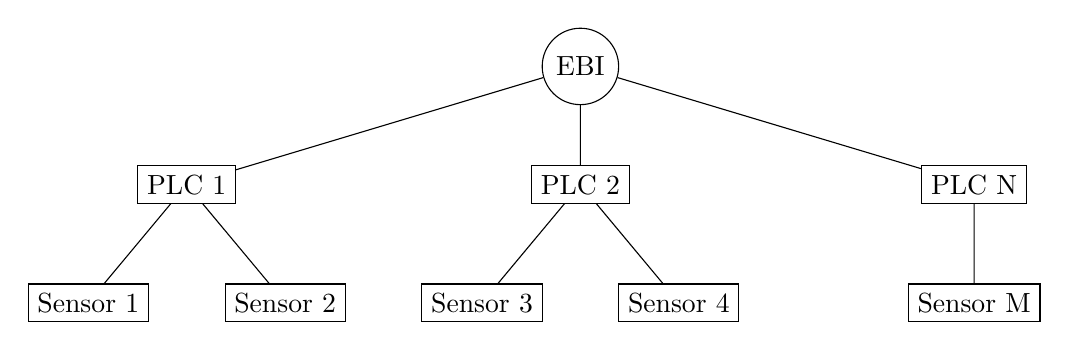
\begin{tikzpicture}[level 1/.style={sibling distance=5cm},
						level 2/.style={sibling distance=2.5cm}]
		\node[circle,draw]{EBI}
			child{
				node[rectangle,draw]{PLC 1}
					child[rectangle,draw]{node[rectangle,draw]{Sensor 1}}
					child[rectangle,draw]{node[rectangle,draw]{Sensor 2}}
				}
			child{
				node[rectangle,draw]{PLC 2}
					child{node[rectangle,draw]{Sensor 3}}
					child{node[rectangle,draw]{Sensor 4}}
				}
			child{
				node[rectangle,draw]{PLC N}
				child{node[rectangle,draw]{Sensor M}}
				}
		;
	\end{tikzpicture}
	\caption{Red industrial Gador.}
	\label{fig:redGador}
\end{figure}


\section{Introducción técnica}
\label{ch1IntroduccionTecnica}

% Presentación modelo de capas IoT
El proyecto realizado presentó una serie de desafíos a resolver, siendo el primero de ellos la variedad de tecnologías involucradas, tanto en la problemática a manipular como en la solución a implementar. Para introducir orden en la variedad de conocimientos que forman parte del sistema desarrollado, se introduce un \emph{modelo de capas de Internet de las cosas (IoT)}. El modelo tiene la ventaja que separa los temas en categorías relacionadas con la función o servicio que prestan en la solución, de la misma manera, cuando se habla de la biología humana y sus múltiples partes y órganos al utilizar el modelo de sistemas del cuerpo humano. 

% Enumeración de las capas y una breve descripción de cada una
El modelo de capas seleccionado separa los conocimientos en cinco categorías, las cuales son las capas de negocio, aplicación, procesamiento, red y percepción.
La capa de negocio agrupa todo lo relacionado con las reglas y el control del sistema, esto incluye supervisar el tráfico de información, verificar el estado de los equipos u otorgar permisos a los usuarios para interactuar con el programa.
La capa de aplicación relaciona todas las tecnologías que se encargan de interactuar con el usuario final, es lo que las personas pueden ver como el sistema.
La capa de procesamiento agrupa los conocimientos cuya responsabilidad es almacenar y analizar los datos que se generan.
La capa de red tiene la finalidad de interconectar los dispositivos para permitir el flujo de datos entre todas las partes involucradas.
Finalmente la capa de percepción se refiere a todos los artefactos que manipulan o miden algo que se encuentra en el ambiente, como un sensor o un actuador. Este modelo se encuentra resumido en la tabla \ref{tab:modeloCapas}.

\begin{table}[h]
	\centering
	\begin{tabular}{c|c}
		Capa          & Función                                  \\ \hline
		Negocio       & Establecer reglas y controlar el sistema \\
		Aplicación    & Interactuar con el usuario               \\
		Procesamiento & Almacenar y analizar los datos obtenidos \\
		Red           & Transportar los datos entre dispositivos \\
		Percepción    & Realizar mediciones o acciones en planta \\
	\end{tabular}
	\caption{\label{tab:modeloCapas}Modelo de capas IoT.}
\end{table}

% Capa de negocios
Dependiendo del modelo viabilidad económica de un sistema y de como fue desplegado, la capa de negocio puede tener una funcionalidad contable y calcular los costos de operación.
Esta capa puede ser la encargada de determinar y generar la facturación para cobrarle a los usuarios de la aplicación, como así también, de resolver operaciones de transferencia de dinero. La interacción en este nivel es con el personal que administra un sistema, se determina que permisos tiene cada usuario para manipular los servicios ofrecidos y se lleva adelante el registro de acciones y eventos relevantes para el normal funcionamiento del programa.

% Capa de aplicación

% Capa de procesamiento

% Capa de red
		
\begin{figure}[h]
	\centering
	\begin{tikzpicture}
		\tikzstyle{broker} = [circle,draw=black]
		\tikzstyle{publish} = [rectangle,draw=black]
		\tikzstyle{subscribe} = [rectangle,draw=black]
		\tikzstyle{flecha} = [->,very thick]

		\node[publish] (p) {Sensor};
		\node[broker,right=of p] (b) {Broker};
		\node[subscribe, right=of b] (s2)	{Cliente 2};
		\node[subscribe,above=of s2] (s1) {Cliente 1};
		\node[subscribe, below=of s2] (s3) {Cliente 3};

		\draw[flecha] (p) edge (b);
		\draw[flecha] (b) edge (s1);
		\draw[flecha] (b) edge (s3);			
	\end{tikzpicture}
	\caption{Ejemplo de comunicación MQTT.}
	\label{fig:mqttEjemplo}
\end{figure}

% Capa de percepción

% Despliegue de una solución


\section{Estado del arte}
\label{ch1EstadoDelArte}

\begin{figure}[h]
	\centering
	\begin{tikzpicture}		
		\tikzstyle{block} = [rectangle,draw=black]
				
		\node[block] (r) {Router};
		\node[below=of r] (aux) {};
		\node[block,right=of aux] (c) {Config};
		\node[block,below=of aux] (s1) {Shard 3};
		\node[block,left=of s1] (s2) {Shard 2};
		\node[block,left=of s2] (s3) {Shard 1};
				
		\draw (r)--(s1);
		\draw (s2)|-(c);
		\draw (s3)|-(aux);
		\draw (c)--(aux);		
	\end{tikzpicture}
	\caption{Arquitectura de datos de alta disponibilidad.}
	\label{fig:mongodb}
\end{figure}


\section{Objetivos y alcance}
\label{objetivos}
	
\begin{figure}[h]
	\centering
	\begin{tikzpicture}			
		\tikzstyle{block} = [rectangle,draw=black]
				
		\node[block] (s1) {Sensor 1};
		\node[block,right=of s1] (s2) {Sensor 2};
		\node[block,right=of s2] (s3) {Sensor 3};
		\node[block,right=of s3] (s4) {Sensor 4};
		\node[block,right=of s4] (sn) {Sensor n};

		\node[block,below=of s2] (a1) {Agregación 1};
		\node[block,below=of s4] (a2) {Agregación 2};

		\node[below=of s1] (aux1) {};
		\node[below=of s3] (aux3) {};
		\node[below=of sn] (auxn) {};

		\node[below=of aux1] (tcp1) {};
		\node[below=of a1] (tcp2) {};
		\node[below=of aux3] (tcp3) {TCP/IP};
		\node[below=of a2] (tcp4) {};
		\node[below=of auxn] (tcpn) {};

		\node[block, below=of tcp2] (ebi) {EBI};
		\node[block, below=of tcp4] (nodos) {Nodos};

		\draw (tcp1)--(tcpn);
		\draw (ebi)--(a1);
		\draw (nodos)--(a2);
				
		\draw (s1)--(a1);
		\draw (s2)--(a1);
		\draw (s3)--(a1);

		\draw (s4)--(a2);
		\draw (sn)--(a2);		
	\end{tikzpicture}
	\caption{Esquema del proyecto.}
	\label{fig:esquemaProyecto}
\end{figure}
	
\begin{itemize}
	\item Debe integrarse a la infraestructura de Gador S.A. sin generar conflictos en otros sistemas.
	\item Debe crear tramas en el formato \emph{Enterprise Buildings Integrator} y enviarlas al servidor.
	\item Debe interpretar eventuales mensajes del servidor \emph{Honeywell}.
	\item Debe interpretar los mensajes de los sensores.
	\item Debe poder cambiar la frecuencia de lectura de mediciones.
	\item Debe poseer la capacidad de gestionar los ingresos de usuarios de forma segura.
	\item Debe permitir que por lo menos 5 (cinco) usuarios accedan al sistema simultáneamente.
	\item Debe presentar una interfaz donde se monitoree el estado de los sensores
	\item Debe permitir elegir un sensor en particular para editarlo.
	\item Debe poseer un módulo de gestión de usuarios.
	\item Debe ser compatible con ordenadores de escritorio y \emph{smartphones}.
	\item Las contraseñas no persistirán como texto plano.
	\item Debe persistir todas las modificaciones realizadas a la configuración de los sensores.
	\item Debe persistir las mediciones obtenidas.
\end{itemize}